\documentclass[fr]{../../../../../../eplexam}
\usepackage[utf8]{inputenc}
\usepackage{listings}
\usepackage{float}
\usepackage{mathtools}
\usepackage{tikz}
\usepackage{enumitem}
\usepackage{lipsum}
\usepackage{graphicx}
\usepackage{caption}
\usepackage{multicol}

\definecolor{mGreen}{rgb}{0,0.6,0}
\definecolor{mGray}{rgb}{0.5,0.5,0.5}
\definecolor{mPurple}{rgb}{0.58,0,0.82}
\definecolor{backgroundColour}{rgb}{0.95,0.95,0.92}
\lstdefinestyle{CStyle}{
    backgroundcolor=\color{backgroundColour},   
    commentstyle=\color{mGreen},
    keywordstyle=\color{magenta},
    numberstyle=\tiny\color{mGray},
    stringstyle=\color{mPurple},
    basicstyle=\footnotesize,
    breakatwhitespace=false,         
    breaklines=true,                 
    captionpos=b,                    
    keepspaces=true,                 
    numbers=left,                    
    numbersep=5pt,                  
    showspaces=false,                
    showstringspaces=false,
    showtabs=false,                  
    tabsize=2,
    language=C
}



\hypertitle{Systèmes informatiques}{4}{SINF}{1252}{2017}{Juin}
{Quentin Dessain}
{Olivier Bonaventure}


\section{Exécution conditionnelle [4 points]}
Le shell \texttt{bash} permet l'exécution conditionnelle de commandes. Celle-ci est décrite comme suit dans la page de manuel de \texttt{bash}:

\vspace{0.2cm}
\texttt{An OR list has the form}

\vspace{0.05cm}
\texttt{command1} $\vert\vert$ \texttt{command2}

\vspace{0.05cm}
\texttt{command2 is executed if and only if command1 returns a non-zero exit status.The return status of AND and OR lists is the exit status of the last command executed in the list.}
\vspace{0.01cm}

Expliquez en détails \textbf{tous} les appels systèmes utilisés \textbf{par le shell} lors de l'éxecution de la ligne de commandes bash suivante:
\vspace{0.01cm}

/bin/prog \textgreater/tmp/t  $\vert\vert$ /bin/prog2

\begin{solution}

\begin{center}
  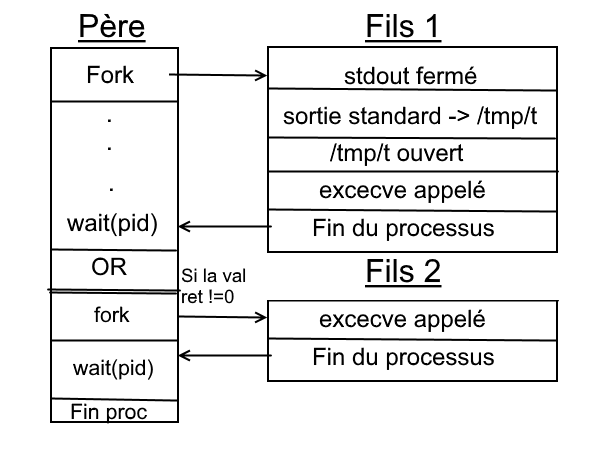
\includegraphics[width=0.6 \textwidth]{latex.png}  
\end{center}

Pour le processus père:
\begin{itemize}
\item Un appel système vers \texttt{fork} est effectué. Ce qui a pour effet de créer un processus fils (processus fils 1).
    \item Un appel vers wait(pid) "bloque" le processus père tant que le fils n'est pas terminé.
    \item La valeur de retour du fils est testée. Si la valeur retournée est différente de zéro, un nouveau processus fils (processus fils 2) est créé.
    \item Si un nouveau processus fils est créé, un appel vers wait(pid) "bloque" le processus père tant que le fils n'est pas terminé. 
\end{itemize}

Pour le processus fils 1:
\begin{itemize}

\item Une fois le processus fils créé, la sortie standard \texttt{stdout} est fermée. 

\item Ensuite la sortie standard du processus fils est redirigé vers le fichier /tmp/t. Si ce dernier n'existait pas, il est créé. Si il existait déjà, il est remit à zéro.

\item Le fichier /tmp/t est ouvert afin de pouvoir ecrire dedans.

\item excecve est appélé et le processus situé dans /bin/prog est lancé.

\item Le processus se termine. (pas d'appel système ? quid de la nouvelle sortie standard ? Elle est fermé ?)

\end{itemize}



Pour le processus fils 2:
\begin{itemize}
    \item excecve est appélé et le processus situé dans /bin/prog2 est lancé.
\end{itemize}



\end{solution}
\section{Mémoire virtuelle [3 points]}


Considérons un processus qui s'exécute sur un ordinateur utilisant la mémoire virtuelle. Pour simplifier, supposons que ce processus utilise une page pour son segment de code, une page pour ses variables globales, une page pour son heap et une page pour son stack. Ce processus dans sa fonction \texttt{main} exécute les lignes suivantes:

\begin{lstlisting}[style=CStyle]
int main(int argc, char** argv){
int *ptr =(int *) malloc(sizeof(int));
*ptr = 1252;
}
\end{lstlisting}


\begin{itemize}


\item[$\bullet$] Expliquez l'organisation du processus en mémoire et indiquez dans quelles zones se trouvent le code des fonctions \texttt{main} et \texttt{malloc}, la variable \texttt{*ptr} et la zone mémoire retournée par malloc.

\begin{solution}

\begin{multicols}{2}
    \begin{center}
         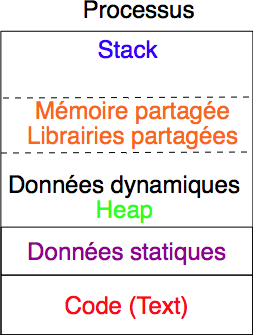
\includegraphics[width=0.4 \textwidth]{orgMemoire.png}
          \captionof{figure}{Organisation en mémoire d’un processus} 
     \end{center}
    \begin{center}
         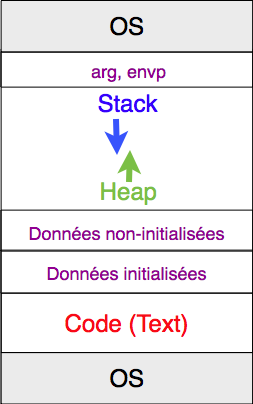
\includegraphics[width=0.3 \textwidth]{figures-001-c.png}
          \captionof{figure}{Organisation d’un programme Linux en mémoire} 
     \end{center}
\end{multicols}


C’est dans le \textbf{segment text} que sont stockées toutes les instructions qui sont exécutées par le micro-processeur.
Il est généralement considéré par l’OS comme étant uniquement
accessible en lecture. C’est dans le segment text qu’on retrouvera les instructions de langage machine correspondant aux fonctions de calcul et d’affichage du programme.\par 
Le code des fcts \texttt{main} et \texttt{malloc} se trouve donc ici.
\newline

C’est dans la \textbf{pile} (\textbf{stack)} que le processus va stocker l’ensemble des variables locales mais
également les valeurs de retour de toutes les fonctions qui sont appelées. Cette zone est gérée comme
une pile (d’où son nom) avec un fonctionnement de type LIFO (Last Input, First Output). À chaque
fois qu’une fonction est appelée elle est placée sur la pile ainsi que ses arguments. Les variables locales
le sont également. Durant son exécution, une fonction accède donc à ses variables locales sur la pile sans
interférer avec les variables locales de l’exécution des autres fonctions. \par
La variable \texttt{*ptr} est placé sur la pile.
\newline

Le \textbf{tas} (ou \textbf{heap}) est une des deux zones dans laquelle un
programme peut obtenir de la mémoire supplémentaire pour stocker de l’information. L’OS mémorise
pour chaque processus en cours d’exécution, la limite supérieure de son heap. Et permet à un processus
de modifier la taille de son heap. En C, la plupart des processus allouent et libèrent de la mémoire en utilisant les
fonctions malloc et free qui font partie de la librairie standard.\par
La zone de mémoire retourné par malloc est donc située sur le heap.
\newline

Le segment des données initialisées contient l’ensemble des données et chaînes de caractères qui sont utilisées
dans le programme. Ce segment contient 2 types de données :
— l’ensemble des variables globales qui sont explicitement initialisées
par le programme ou initialisée à 0 par le compilateur.
— les constantes et chaînes de caractères utilisées par le programme.
\newline

Le segment des données non-initialisées est réservé aux variables non initialisées. Cette zone en mémoire est initialisée à zéro par l’OS au démarrage du programme.

\end{solution}

\item[$\bullet$] Dessinez la table des pages de ce processus avec les valeurs des différents drapeaux au démarrage du processus. Expliquez le rôle de ces drapeaux.

\begin{solution}
\begin{table}[H]
\centering
\label{my-label}
\begin{tabular}{|c|l|l|l|l|l|}
\hline
Page & \multicolumn{1}{c|}{\begin{tabular}[c]{@{}c@{}}Bit de \\ référence\end{tabular}} & \multicolumn{1}{c|}{\begin{tabular}[c]{@{}c@{}}Bit de \\ modification\\ (dirty bit)\end{tabular}} & \multicolumn{1}{c|}{\begin{tabular}[c]{@{}c@{}}Bit de \\ permission \\ (R-W-X)\end{tabular}} & \multicolumn{1}{c|}{\begin{tabular}[c]{@{}c@{}}Bit de \\ validité\end{tabular}} & \multicolumn{1}{c|}{\begin{tabular}[c]{@{}c@{}}Localisation \\ de la Page\end{tabular}} \\ \hline
\multicolumn{6}{|c|}{Etat à la ligne 1 du code} \\ \hline
Segment Text & T & F & R - X & Inchangé &  \\ \hline
Variables Globales & F & F & R - W & Inchangé &  \\ \hline
Heap & T & F & R - W & Inchangé &  \\ \hline
Stack & T & F & R -W & Inchangé &  \\ \hline
\multicolumn{6}{|c|}{Etat à la ligne 2 du code} \\ \hline
Segment Text & T & F & R - X & Inchangé &  \\ \hline
Variables Globales & F & F & R - W & Inchangé &  \\ \hline
Heap & T & T & R - W & Inchangé &  \\ \hline
Stack & T & T & R - W & Inchangé &  \\ \hline
\multicolumn{6}{|c|}{Etat à la ligne 3 du code} \\ \hline
Segment Text & T & F & R - X & Inchangé &  \\ \hline
Variables Globales & F & F & R - W & Inchangé &  \\ \hline
Heap & T & T & R - W & Inchangé &  \\ \hline
Stack & T & T & R - W & Inchangé &  \\ \hline
\end{tabular}
\end{table}

\begin{itemize}
    \item Bit de référence: indique si la page a été lue
    \item Bit de modification (dirty bit): indique si la page a été lue
    \item Bit de permission (R,W,X): indique si la page est accessible en lecture / écriture / exécution
    \item Bit de validité: indique si la page est présente en RAM ou sur l’espace d’échange (swap)
\end{itemize}

\end{solution}

\end{itemize}
\newpage
\section{Algorithme de Peterson [3 points]}

Un site Internet propose l'implémentation suivante pour résoudre le problème de l'exclusion mutuelle en C. Cette implémentation est-elle correcte? Si oui, justifiez en détails l'absence de deadlock et de violation de section critique. Si non, expliquez via un exemple pourquoi elle ne fonctionne pas et proposez une correction en utilisant les mêmes variables.

\begin{lstlisting}[style=CStyle]

// Initialisation
int a=false;
int b=false;
int c=0;

// thread 0
a=true;
c=0;

while(b || (c==1) ) {}
section_critique();
a=false;

//thread 1
b=true;
c=1;
while(a || (c==0) ) {}
section_critique();
b=false;

\end{lstlisting}

\begin{solution}
Cette implémentation est incorrecte et conduit à un deadlock.
\newline

Exemple: \par Les 2 premières lignes du premier threads sont executées suivit des 3 premières lignes du deuxième threads. Ensuite la troisième ligne du premier thread est éxecutée.
\par
Les thread 1 et 2 sont alors tous les deux bloqué dans une boucle infinie sans qu'un thread puisse libérer l'autre. On est donc bien fasse à un deadlock
\end{solution}

\end{document}
